

\documentclass{article}
\usepackage[utf8]{inputenc}
\usepackage{authblk}
\usepackage{setspace}
\usepackage[margin=1.25in]{geometry}
\usepackage{graphicx}
\graphicspath{ {./figures/} }
\usepackage{subcaption}
\usepackage{amsmath}
\usepackage{algorithm}
\usepackage{amssymb}
\usepackage{algpseudocode}
\usepackage{booktabs}
\usepackage{array}
\usepackage{tikz}
\usetikzlibrary{arrows.meta,positioning,calc}
\usepackage{pgfplots}
\pgfplotsset{compat=1.17}

%%%%%% Bibliography %%%%%%
\usepackage[style=nejm,
citestyle=numeric-comp,
sorting=none,
backend=bibtex]{biblatex}
\addbibresource{bib1.bib}
\setcounter{biburlnumpenalty}{9000}
\setcounter{biburllcpenalty}{7000}
\setcounter{biburlucpenalty}{8000}
\renewcommand*{\bibfont}{\raggedright}

\DeclareMathOperator*{\argmax}{arg\,max}
\DeclareMathOperator*{\argmin}{arg\,min}
\newcommand{\cond}[1]{\textsf{#1}}

%%%%%% Title %%%%%%
\title{Semi-supervised Conditional Agents}

%%%%%% Authors %%%%%%
% Corresponding author: add an asterisk and an e-mail address before submission.
\author{Alfred Ricker}

%%%%%% Date %%%%%%
\date{}

%%%%%% Spacing %%%%%%
\onehalfspacing

\begin{document}

\maketitle

%%%%%% Abstract %%%%%%
\begin{abstract}
Can an agent reach goals that need long chains of steps by reasoning backward over conditions it has learned from its own experience, instead of simulating futures and choosing the one with the most reward? World models learned from pixels usually plan by imagined rollouts and learn from reward, which makes long, sparsely rewarded tasks expensive. We describe a conditional agent built on three general parts: a belief state made of tokens, each an appearance vector and a position; an effect model that predicts what an action does to the tokens it touches, by a similarity-weighted vote over stored experience with a neural network as prior; and a planner that regresses from a goal condition through the conditions under which actions have their effects, as in classical means-ends analysis, but with each action's preconditions and effects learned from experience rather than written by hand. A held intention, value iteration over the agent's own believed map, and a rule that acts where an outcome is least known complete the agent. Learning only from about 3.2 million steps of reward-free random play per environment, the agent solved 200 of 200 episodes of MiniGrid's DoorKey-8x8, 100 of 100 of BlockedUnlockPickup and 30 of 30 of ObstructedMaze-Full, plus 100 of 100 further ObstructedMaze-Full layouts, at 2 to 12 milliseconds per step on a CPU. The perception adapter and several declared priors are still specific to MiniGrid, and we list them with the work under way to remove them. Planning over learned conditions is a sample-efficient and inspectable alternative to planning by imagined rollouts.
\end{abstract}

%%%%%% Main Text %%%%%%

\section{Introduction}

Modern machine learning struggles with planning over long time horizons. World models are an attempt to form compressed spatiotemporal representations of an environment and to use them for reinforcement learning \cite{Schmidhuber1990,Ha2018}. An agent with such a model can learn from imagined experience as well as real experience \cite{Sutton1991}. Simulation planners such as PlaNet and Dreamer \cite{Hafner2019,Hafner2020,Hafner2025} and MuZero \cite{Schrittwieser2020} roll a learned latent dynamics model forward and choose actions by the reward of the imagined futures. A related line of work, the joint-embedding predictive architecture (JEPA), holds that predictions should be made in the latent space itself, so that the factors a pixel decoder would have to reproduce, but which do not matter for the task, can be compressed out \cite{LeCun2022,Assran2023}.

Planning by rollouts has two costs when tasks are long and rewards are sparse. Rewards must first be found by exploration before they can shape either the model or the policy. And the number of imagined trajectories needed to find a good one grows with the horizon. MiniGrid's ObstructedMaze-Full \cite{ChevalierBoisvert2023} is an example. The agent must find keys hidden in boxes, move balls that block doors, unlock doors of the matching colour across a maze of rooms, and pick up a target ball, with a single reward at the end. In one comparison of six reinforcement-learning methods on the original version of this task, only one, NovelD, learned to solve it; ICM, RND, RIDE, AMIGo and IMPALA all scored zero \cite{Zhang2021}.

Instead of simulating probable futures and choosing the one with maximum reward, the conditional agent takes an approach inspired by classical planning and by cognition \cite{Lake2017}. When we bake a cake or clean a room, we have an end condition that is either true or false: the cake is baked, the room is clean. To reach it, we reason about the conditions that make it possible. We know from experience that a cake needs the right ingredients, mixed and put in a hot oven. Each of these conditions is itself a goal with its own conditions: to have the ingredients, we must buy them, and to buy them we must be at the shop. The chain runs backward from the goal to an action we can take now, and only the conditions that matter for the goal are ever considered. This is means-ends analysis, the core of the General Problem Solver and of STRIPS \cite{Newell1972,Fikes1971}. Its weakness was that the operators, each action's preconditions and effects, were written by hand. Later work learned symbolic operators from data, usually from supplied object features or predicates \cite{Pasula2007,Kansky2017,Silver2023}, or planned in a learned latent space with a classical planner \cite{Asai2018}.

In this paper the operators are not written and not given as symbols. The agent learns what an action does to the tokens it touches from its own reward-free experience, by a similarity-weighted vote over stored tries with a neural network as prior. A condition is then any predicate over the agent's belief that a learned effect can make true: holding a given object, a given token being passable, facing a token. Planning works backward over these conditions, and a condition that is not yet true becomes a subgoal. We call the agent semi-supervised because its experience carries no labels and no rewards. The only supervision is the goal condition it is given and the environment's signal that an episode has ended.

Our contributions are:
\begin{itemize}
    \item a belief state of tokens, each an appearance vector and a position, in which the agent's moves are rigid transformations fitted from its own observations (Section~\ref{sec:belief});
    \item an effect model that predicts whether an action changes the token it acts on and the token the agent carries, what each becomes and how certain that is, from an exemplar vote with a network prior, and that one failed try in the current episode corrects (Section~\ref{sec:effects});
    \item a planner that regresses over learned conditions, checks each need in the situation that the predicted effects produce, and orders competing needs by asking itself whether one can still be reached after the other (Section~\ref{sec:planning});
    \item commitment to a chain of conditions between steps, and a single rule for acting when no plan exists: act where the predicted outcome is least certain (Sections~\ref{sec:intention} and~\ref{sec:noplan});
    \item results on three MiniGrid environments of increasing difficulty (Figure~\ref{fig:tiers}), with the contribution of each component measured on paired seeds as it was added, and an audit of which assumptions are still specific to MiniGrid.
\end{itemize}

\begin{figure}[t]
    \centering
    \begin{subfigure}{0.27\textwidth}
        \centering
        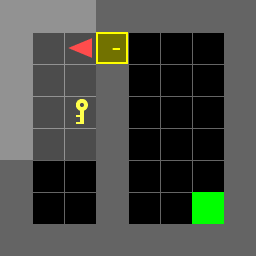
\includegraphics[width=\textwidth]{tier1}
        \caption{\label{fig:tiers:a}}
    \end{subfigure}\hfill
    \begin{subfigure}{0.34\textwidth}
        \centering
        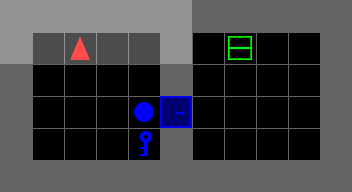
\includegraphics[width=\textwidth]{tier2}
        \caption{\label{fig:tiers:b}}
    \end{subfigure}\hfill
    \begin{subfigure}{0.31\textwidth}
        \centering
        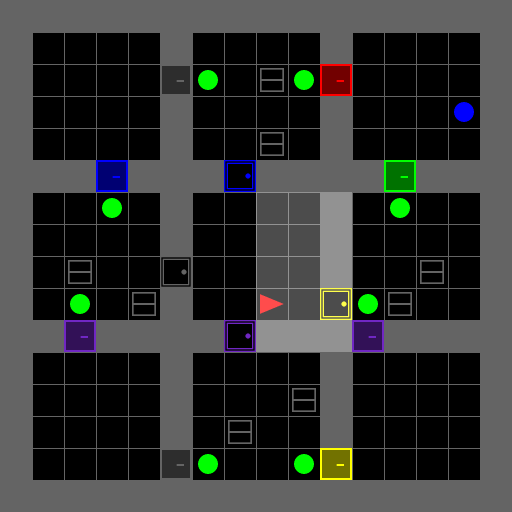
\includegraphics[width=\textwidth]{tier3}
        \caption{\label{fig:tiers:c}}
    \end{subfigure}
    \caption{The three evaluation environments, each shown at its first test seed. (\subref{fig:tiers:a}) DoorKey-8x8: pick up the key, unlock the door and reach the goal square. (\subref{fig:tiers:b}) BlockedUnlockPickup: move the ball that blocks the door, fetch the key, unlock the door and pick up the box. (\subref{fig:tiers:c}) ObstructedMaze-Full: keys are hidden in boxes, balls block doors and locked doors connect nine rooms; the target is the blue ball. The agent is the red triangle. It sees only the $7\times7$ window ahead of it (shaded), and walls and closed doors hide what lies behind them.}
    \label{fig:tiers}
\end{figure}

\section{Method}
\label{sec:method}

\subsection{Overview}

Figure~\ref{fig:architecture} shows the agent. Its parts can be read as four kinds of memory, following the complementary learning systems account of human memory and the division of long-term memory into declarative and procedural kinds \cite{McClelland1995,Kumaran2016,Squire2004}:
\begin{itemize}
    \item \textbf{Working memory} holds the believed scene, the goal and the chain of conditions the agent is pursuing.
    \item \textbf{Event memory} holds every stored try: an action, the tokens it read, and what changed.
    \item \textbf{Structure} is held by networks trained offline: the encoder that turns image patches into vectors, and two networks that serve as priors where stored experience is sparse.
    \item \textbf{Procedural memory} is the computed walking routine, which runs without deliberation.
\end{itemize}
All four read and write the same vectors, the encoder's. Deliberation, in the sense of System 2 \cite{Kahneman2011}, is the backward search over conditions. It runs only when the held chain of conditions stops answering.

\begin{figure}[t]
    \centering
    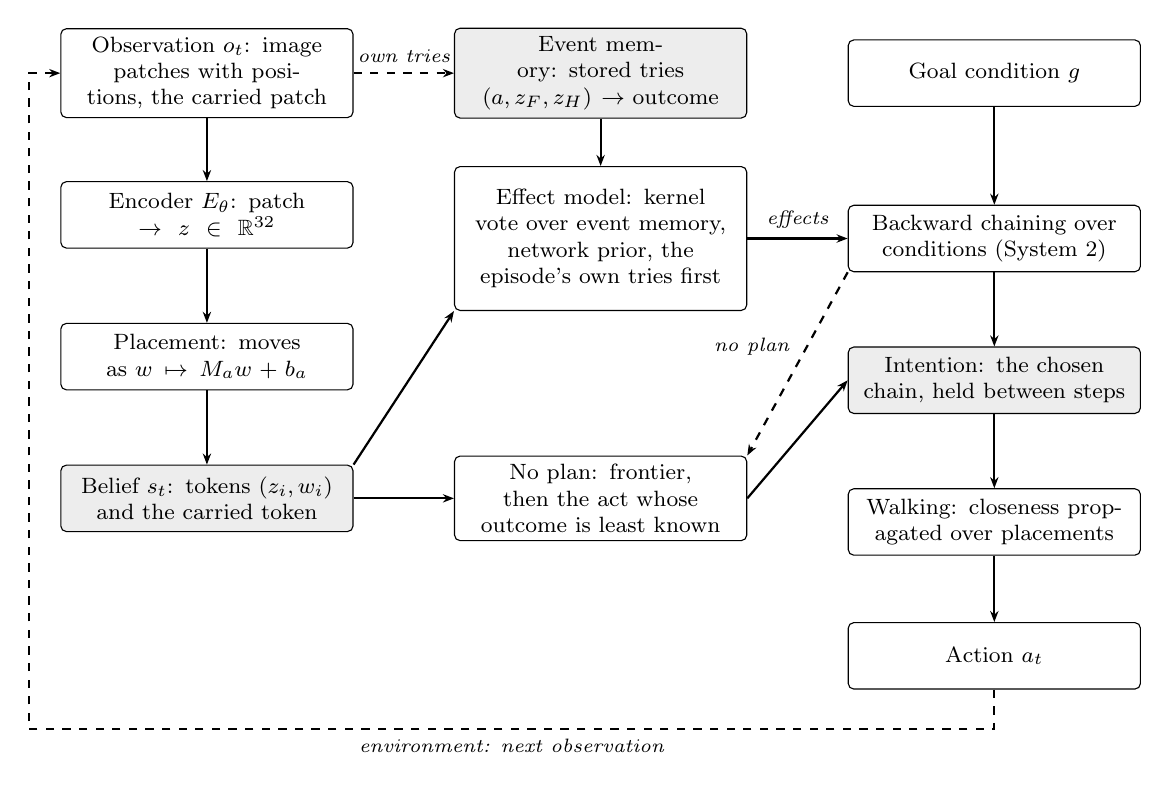
\begin{tikzpicture}[
        font=\footnotesize,
        box/.style={draw, rounded corners=2pt, align=center, text width=3.5cm, minimum height=2.4em, inner sep=3pt, fill=white},
        mem/.style={box, fill=black!7},
        arr/.style={-{Stealth[length=4pt]}, thick},
        lab/.style={font=\scriptsize\itshape, align=center}
    ]
        \node[box] (obs) at (0,0) {Observation $o_t$: image patches with positions, the carried patch};
        \node[box] (enc) at (0,-1.8) {Encoder $E_\theta$: patch $\to z\in\mathbb{R}^{32}$};
        \node[box] (place) at (0,-3.6) {Placement: moves as $w\mapsto M_a w+b_a$};
        \node[mem] (belief) at (0,-5.4) {Belief $s_t$: tokens $(z_i, w_i)$ and the carried token};
        \node[mem] (events) at (5.0,0) {Event memory: stored tries $(a, z_F, z_H)\to$ outcome};
        \node[box, minimum height=5.2em] (effect) at (5.0,-2.1) {Effect model: kernel vote over event memory, network prior, the episode's own tries first};
        \node[box] (noplan) at (5.0,-5.4) {No plan: frontier, then the act whose outcome is least known};
        \node[box] (goal) at (10.0,0) {Goal condition $g$};
        \node[box] (plan) at (10.0,-2.1) {Backward chaining over conditions (System 2)};
        \node[mem] (intent) at (10.0,-3.9) {Intention: the chosen chain, held between steps};
        \node[box] (walk) at (10.0,-5.7) {Walking: closeness propagated over placements};
        \node[box] (act) at (10.0,-7.4) {Action $a_t$};
        \draw[arr] (obs) -- (enc);
        \draw[arr] (enc) -- (place);
        \draw[arr] (place) -- (belief);
        \draw[arr] (events) -- (effect);
        \draw[arr] (belief.north east) -- (effect.south west);
        \draw[arr] (goal) -- (plan);
        \draw[arr] (effect.east) -- node[lab, above]{effects} (plan.west);
        \draw[arr] (plan) -- (intent);
        \draw[arr] (intent) -- (walk);
        \draw[arr] (walk) -- (act);
        \draw[arr, dashed] (plan.south west) -- node[lab, above left=-1pt]{no plan} (noplan.north east);
        \draw[arr] (noplan.east) -- (intent.west);
        \draw[arr] (belief.east) -- (noplan.west);
        \draw[arr, dashed] (obs.east) -- node[lab, above]{own tries} (events.west);
        \draw[arr, dashed] (act.south) -- ++(0,-0.5) -| node[lab, pos=0.25, below]{environment: next observation} ($(obs.west)+(-0.4,0)$) -- (obs.west);
    \end{tikzpicture}
    \caption{Architecture of the conditional agent. Shaded boxes are memories. Each step, the observation is encoded and placed into the belief, a set of tokens. The effect model predicts what an interaction does to the token at the action's locus and to the carried token. The planner works backward from the goal condition through the conditions under which actions have their effects, down to a condition the agent can meet by walking or by acting now. The chosen chain of conditions is held as an intention until a trigger calls for deliberation. When no plan exists, the agent explores or acts where the predicted outcome is least certain. Every try's outcome is added to event memory as one of the episode's own tries.}
    \label{fig:architecture}
\end{figure}

\subsection{Problem setting}

At each step $t$ the agent receives an observation $o_t$: a set of image patches, each with a position relative to the agent, plus the patch of the object it carries, if any. It chooses an action $a_t$ from a finite set $\mathcal{A}$. In MiniGrid a patch is one $8\times8$ grid cell, positions are offsets on the grid, and $\mathcal{A}$ has six actions: turn left, turn right, move forward, pick up, drop and toggle. Toggle opens and closes doors, unlocks a door when the matching key is carried, and opens boxes.

Before the test episodes the agent has a dataset $\mathcal{D}$ of its own experience, collected by a uniformly random policy without reward. At test time it is given a goal condition $g$, a predicate on its belief, and must make $g$ true. No reward is used for learning. The environment's termination signal is the only outcome it reports, and the agent stores it like any other outcome.

\subsection{Perception: patches to vectors}
\label{sec:encoder}

An encoder $E_\theta$ maps an image patch $x$ to a vector $z\in\mathbb{R}^{32}$. Two convolutional layers and a linear layer give $u\in\mathbb{R}^{32}$, which is cut into four pieces of eight, each normalised to unit length:
\begin{equation} \label{eq:encoder}
    z = E_\theta(x) = \left(\frac{u_1}{\|u_1\|_2}, \dots, \frac{u_4}{\|u_4\|_2}\right).
\end{equation}
There is no decoder and no pixel reconstruction. The encoder is trained, in the JEPA spirit, to make the consequences of actions predictable in its own space. A transition network $T_a$ predicts, for each interaction $a$, the vectors of the front and carried patches after the action from their vectors before, $(\hat z'_F, \hat z'_H) = T_a(z_F, z_H)$. The target is an exponential moving average $\bar\theta$ of the encoder's own weights, as in BYOL \cite{Grill2020}:
\begin{equation} \label{eq:trans}
    \mathcal{L}_{\text{trans}} = \sum_{a}\mathbb{E}\left[\big\|\hat z'_F - \mathrm{sg}\,E_{\bar\theta}(x'_F)\big\|^2 + \big\|\hat z'_H - \mathrm{sg}\,E_{\bar\theta}(x'_H)\big\|^2\right].
\end{equation}
Here $x_F$ and $x_H$ are the patch at the action's locus (the cell ahead) and the carried patch, primes denote the next step, and $\mathrm{sg}$ stops the gradient. Two margins keep the space from collapsing, much as the hinge term of contrastive structured world models does \cite{Kipf2020}. Both use a noise ceiling $\tau_{\text{pix}}$ that the agent measures itself: 1.25 times the largest mean absolute pixel difference between two views of an untouched patch under independent noise. Patches that differ by more than $\tau_{\text{pix}}$ are visibly different. The two margins are:
\begin{align}
    \mathcal{L}_{\text{vis}} &= \mathbb{E}_{(x,x'):\,d_{\text{pix}}(x,x')>\tau_{\text{pix}}}\max\big(0,\,1-\|E_\theta(x')-E_\theta(x)\|_2\big), \label{eq:vis}\\
    \mathcal{L}_{\text{pair}} &= \mathbb{E}_{i<j:\,d_{\text{pix}}(x_i,x_j)>\tau_{\text{pix}}}\max\big(0,\,0.5-\|E_\theta(x_i)-E_\theta(x_j)\|_2\big). \label{eq:pair}
\end{align}
The first says that a change an action visibly made must move the vector. The second says that visibly different patches must lie apart. A further term, $\mathcal{L}_{\text{view}}$, maps an untouched patch under fresh noise to the same target. A relational term judges whether a key ``fits'' a door only through the difference of their vectors, $r=\|B(z_F-z_H)\|_1$ with $B\in\mathbb{R}^{8\times32}$, on objects of freshly sampled colours. Materials and Methods give the full objective.

The same vectors are read at two resolutions. As \emph{vectors}, they give graded similarity. As \emph{identity codes}, each piece is assigned to the nearest class within that piece's measured noise scale, so two patches share a code exactly when they are the same up to noise. Codes are names, not labels: what a code means is never engineered.

\subsection{Belief: tokens, moves and placement}
\label{sec:belief}

The belief is a set of tokens \cite{Dosovitskiy2021,Locatello2020}. Each token $i$ has a \emph{what}, an appearance vector $f_i\in\mathcal{Z}\cup\{\varnothing\}$ (empty if it has never been seen), and a \emph{where}. One extra token, the carried slot $H$, has a what $f_H$ and no where. A situation is
\begin{equation} \label{eq:situation}
    s = (f, q, e),
\end{equation}
where $f$ assigns a what to every token, $q$ is a placement and $e$ records whether the episode has ended. A placement is a rigid transformation $q=(R_q, t_q)$. It gives every token its where relative to the agent, $w_i = R_q w_i^0 + t_q$, from the token's coordinate $w^0_i$ in the frame of the episode's first view. Moving the agent moves every token alike, so a situation stores one transformation, not a position per token.

\paragraph{Moves are learned transformations.} For each movement action $a$, the agent fits a transformation $w\mapsto M_a w+b_a$ from random play, without being told that the view turns or shifts. It counts, over stored steps with action $a$, how often the appearance at view position $\omega$ before the step determines the appearance at position $\omega'$ after it. A pair $(\omega,\omega')$ is a correspondence when $\omega$'s appearance determines $\omega'$'s in every one of at least 50 observed steps, and $\omega$'s appearance varies. Correspondences are fitted by least squares, trimmed one at a time \cite{Rousseeuw1984}:
\begin{equation} \label{eq:moves}
    (M_a, b_a) = \argmin_{M,b}\sum_{(\omega,\omega')\in K}n_{\omega\omega'}\,\big\|M \omega + b - \omega'\big\|_2^2,
\end{equation}
where positions are vectors in the agent's frame, $n_{\omega\omega'}$ counts the observed steps and $K$ loses its worst-fitting pair until every residual is below half a cell. On all three environments this gives exact quarter turns for left and right and a unit shift for forward, with zero residual.

\paragraph{Placing a view.} The placements reachable by composing the learned moves form a lattice. After action $a_{t-1}$, the agent's new placement is chosen among those the action could lead to: staying put, or the move's result. It is the one whose predicted view best matches the observed one:
\begin{equation} \label{eq:placement}
    q_t = \argmin_{q'\in\{q_{t-1},\,(M_{a}, b_{a})\circ q_{t-1}\}}\ \sum_{\omega\in\mathcal{O}_t}\big[f_{i(q',\omega)}\neq\varnothing\big]\,\big\|z\big(f_{i(q',\omega)}\big) - z(o_{t,\omega})\big\|_1 .
\end{equation}
Here $\mathcal{O}_t$ is the set of observed positions, $i(q',\omega)$ is the token shown at position $\omega$ under placement $q'$, and $z(\cdot)$ is an appearance's vector. Never-seen tokens give no evidence. The observed patches then become the whats of the tokens in view, and every other token keeps the last appearance seen there. A never-seen token is imagined with the commonest appearance of places that enter the view, but it is never treated as passable.

\subsection{The effect model}
\label{sec:effects}

The effect model answers one question for the interaction actions (pick up, drop and toggle in MiniGrid). Given an action $a$, the appearance $u$ of the token at the action's locus and the appearance $h$ of the carried token, it predicts whether each of the two changes and what each becomes. The locus is the place an action acts on. For MiniGrid's interactions it is the cell ahead, a deictic reference in the sense of Pasula et al.~\cite{Pasula2007}. Each query becomes two \emph{instances}, one for the locus token and one for the carried token, and each instance is predicted separately.

\paragraph{An exemplar vote.} Every stored try contributes token instances. Each instance records the token's appearance, its role (locus or carried), the appearances in its context, a label $y\in\{0,1\}$ for whether it changed, and a weight $w$ from the sampling of experience. Instances that agree on the admitted conditions (below) form groups $\gamma$, with total weight $n_\gamma$ and changed weight $m_\gamma$. A query instance $x$ is answered by a similarity-weighted vote, as in exemplar models of memory and categorisation \cite{Medin1978,Nosofsky1986,Hintzman1986} and in kernel regression \cite{Nadaraya1964,Watson1964}:
\begin{equation} \label{eq:vote}
    N_1(x) = \sum_{\gamma:\,D(x,\gamma)<R} e^{-D(x,\gamma)}\,m_\gamma, \qquad N(x) = \sum_{\gamma:\,D(x,\gamma)<R} e^{-D(x,\gamma)}\,n_\gamma ,
\end{equation}
\begin{equation} \label{eq:metric}
    D(x,\gamma) = \sum_{\ell\in\mathcal{C}_a}\frac{\lambda_\ell}{s_\ell}\,d_\ell(x,\gamma).
\end{equation}
Each candidate condition $\ell$ compares one part of the instance: the L1 distance between one 8-number piece of the two tokens' appearances, of one context token's appearance, or whether the roles differ. Each condition's distance is divided by its mean over random pairs, $s_\ell$, and weighted by $\lambda_\ell$. Only the admitted conditions $\mathcal{C}_a$ of action $a$ enter. The radius $R=12$ makes the vote exact in practice: excluded groups weigh less than $e^{-12}$. An index over the admitted columns finds the groups within the radius without scanning the store.

\paragraph{Which conditions matter is learned.} Conditions are admitted greedily, starting from none. Each round adds the condition and weight $\lambda_\ell\in\{0.5,1,\dots,16\}$ that most raise the leave-one-try-out log-likelihood of the stored outcomes. Admission stops when the best gain falls below $\ln 57$, the cost in nats of naming one of the 57 candidate conditions. A condition that never changed an outcome therefore cannot veto a memory. On all three environments most admitted conditions compare pieces of the locus token's appearance and of the carried token's appearance, together with the role. The agent keeps only these and marginalises conditions on other places in view, which costs almost nothing on held-out tries (Results).

\paragraph{A network as prior.} Where stored experience is sparse, the vote defers to a network $p_A$ that attends over a state's tokens \cite{Vaswani2017,Battaglia2018}. It predicts, for every token, the probability that the action changes it. The two are combined as pseudo-counts:
\begin{equation} \label{eq:armc}
    p_C(x) = \frac{N_1(x) + \alpha_a\, p_A(x)}{N(x) + \alpha_a}.
\end{equation}
The weight $\alpha_a$ is fitted per action by leave-one-try-out likelihood. Its fitted value is small (0.01 in eight of nine cases), so the network decides only where no stored instance lies within the radius. For a query $(a,u,h)$, write $p_F$ and $p_H$ for the locus and carried predictions. The four outcome categories (nothing changes, the locus changes, the carried token changes, both change) are taken as independent products, $\pi_C = \big((1-p_F)(1-p_H),\ p_F(1-p_H),\ (1-p_F)p_H,\ p_F p_H\big)$.

\paragraph{The episode's own tries come first.} Let $\boldsymbol{\nu}\in\mathbb{N}^4$ count this episode's own tries of the same $(a,u,h)$ by outcome category. Then
\begin{equation} \label{eq:own}
    \pi = \frac{\boldsymbol{\nu} + \beta_a\,\pi_C}{|\boldsymbol{\nu}| + \beta_a},
\end{equation}
and the predicted category is $\hat{k}=\argmax_k \pi_k$ if $\max_k\pi_k\ge\tfrac12$, otherwise ``nothing changes''. The weight $\beta_a$ is again fitted by leave-one-try-out likelihood on stored experience. The fit reaches the bottom of its grid ($\beta\approx1.2\times10^{-4}$) on every action and environment: in these worlds one try decides. A single failed try, such as toggling a locked door while carrying a key of another colour, therefore corrects the prediction for the rest of the episode.

\paragraph{What a changed token becomes, as a relation.} A stored outcome is not copied literally. For each piece $k$ of the result vector, the agent asks which of four relations best explains the nearest changed instances, weighting each by $\omega_i=e^{-D}w_i$:
\begin{itemize}
    \item \emph{keep} the token's own piece;
    \item \emph{copy} the piece from another token of the try, for example the locus token into the carried slot;
    \item \emph{shift} it by a constant $\delta$;
    \item \emph{set} it to a constant value.
\end{itemize}
The relation with the most support is applied to the query's own tokens. The result is snapped to the nearest known appearance in L1. So ``picking up puts the token at the locus into the carried slot'' holds for a box of a colour that has rarely been picked up, because the relation is \emph{copy from the locus}, not \emph{set to a red box}.

\paragraph{Certainty about the result.} When a relation is \emph{shift} or \emph{set}, the neighbours may disagree about the value. A box, for example, may hold a key of any of six colours. The certainty $\eta(a,u,h)$ is the smallest, over such pieces, of the winning value's share of the neighbour weight. It is 1 when every piece is kept or copied. Section~\ref{sec:noplan} uses it.

\paragraph{Walking onto a token.} Moving forward has its own model of the same form, kept per appearance $v$. The outcomes are: the agent moved, it was blocked, or the episode ended. Their counts $N(v)$ come from stored and own tries:
\begin{equation} \label{eq:walk}
    P(\cdot\mid v) = \frac{N(v) + \beta_F\,\phi(z_v)}{\sum N(v) + \beta_F}.
\end{equation}
Here $\phi$ is a small ensemble of networks that predicts these outcomes from the appearance vector, trained offline on objects of freshly sampled colours. Its fitted weight $\beta_F=10^{-3}$ means it decides only appearances the agent has never walked into, for example a door colour first seen open during an episode. An appearance is \emph{passable} when ``moved'' is its most likely outcome.

\subsection{Conditions and backward chaining}
\label{sec:planning}

A \emph{condition} is a predicate over a situation. Table~\ref{tab:conditions} lists the vocabulary. The five forms are declared; which tokens, carried objects and actions fill them is learned. Every condition is checked against the belief, and every way of making one true comes from a learned model. There is no list of objects, kinds or rules.

\begin{table}[t]
    \caption{The conditions the planner reasons over. $a$ is an action, $u$ an appearance, $j$ a token, $h$ the appearance of a carried token, and $s$ a situation.}
    \centering
    \small
    \begin{tabular}{>{\raggedright\arraybackslash}p{2.6cm} >{\raggedright\arraybackslash}p{5.0cm} >{\raggedright\arraybackslash}p{5.2cm}}
        \toprule
        Condition & Holds in $s$ when & Made true by \\
        \midrule
        \cond{end} & the episode has ended & moving onto an appearance whose predicted forward outcome is ``ended'' \\
        \cond{has}$(h)$ & the carried slot holds $h$ & an interaction whose predicted effect puts $h$ in the carried slot \\
        \cond{walk}$(j)$ & moving onto token $j$ is predicted to succeed & an interaction on $j$ whose predicted result is passable \\
        \cond{face}$(a,u,j)$ & the agent stands on a passable token with token $j$, showing $u$, at the locus of $a$ & walking (Section~\ref{sec:walking}) \\
        \cond{part}$(a,u,j,c)$ & doing $a$ on $u$ at $j$ with the carried token of $s$ is predicted to make $c$ true & an interaction that changes the carried token to one under which $a$ works \\
        \bottomrule
    \end{tabular}
    \label{tab:conditions}
\end{table}

\paragraph{Imagined effects.} Let $\mathrm{Im}(s,a,u,j)$ be the situation the effect model predicts when $a$ is done on token $j$, showing $u$, in $s$. Token $j$ takes its predicted result, the carried slot takes its predicted result, and nothing else changes. If the predicted category is ``nothing changes'', $\mathrm{Im}=\bot$. An action $a$ on $(u,j)$ \emph{achieves} condition $c$ in $s$ when $\mathrm{Im}(s,a,u,j)\neq\bot$ and $c$ holds in it.

\paragraph{Achievers and their needs.} An achiever of $c$ has at most two needs:
\begin{itemize}
    \item a condition on the carried token, \cond{part}$(a,u,j,c)$, when the action works only with another carried token;
    \item facing its token, \cond{face}$(a,u,j)$.
\end{itemize}
The carried tokens worth considering are those under which the action changed something in stored experience or in the episode's own tries. For example, the goal \cond{has}(blue ball) has the achiever ``pick up the blue ball''. In ObstructedMaze-Full, \cond{walk}(door) has the achiever ``toggle the door''. Toggling a locked door with an empty hand is predicted to change nothing, so the achiever's need is \cond{part}(toggle, door, $j$, \cond{walk}): carry something under which toggling opens the door. Its achiever in turn is ``pick up the key of the door's colour''.

\paragraph{Needs are checked in the situations that effects produce.} A need is judged in the situation that imagining the achiever's effect on the present produces, never in a situation pieced together from stored examples. In the example, the agent imagines picking up the key. That gives a situation in which the key is carried and its place is empty. It then imagines toggling the door in that situation and checks that the door becomes passable. Composing imagined effects from the present keeps every hypothetical consistent: a key that has been used cannot be counted twice.

\paragraph{Regression.} Algorithm~\ref{alg:solve} gives the search. It starts from the goal and recurses through unmet needs to a depth of six. A \cond{face} need is the leaf: it is met by walking, or, when the way is blocked, it raises a \cond{walk}$(j)$ condition for the first blocking token on the best route. When a need already holds, the achiever's action is the step to take. Before the action is taken, the agent imagines it and \emph{refuses} it if it would undo a protected condition, one that a pending need relies on. A refusal triggers a re-plan, at most twelve per step. The result is a chain of conditions from the goal down to one action.

\begin{algorithm}[t]
\caption{Backward chaining over learned conditions}
\label{alg:solve}
\begin{algorithmic}[1]
\Function{Solve}{$c, s, d, C, P$} \Comment{condition, situation, depth, chain above, protected}
    \State $\mathcal{X}\gets$ achievers $(a,u,j)$ of $c$ in $s$ whose needs avoid $C\cup\{c\}$
    \For{each group of $\mathcal{X}$ with equal numbers of unmet needs, fewest first}
        \State $\Pi\gets\emptyset$
        \For{each achiever $(a,u,j)$ in the group, with needs $\mathcal{N}$}
            \If{every need in $\mathcal{N}$ holds in $s$}
                \State $s'\gets$ the predicted step of $a$ in $s$
                \If{$c$ holds in $s'$ and every $p\in P$ that holds in $s$ holds in $s'$}
                    \State add the plan ``do $a$'' to $\Pi$
                \Else
                    \State refuse $a$ here and re-plan
                \EndIf
            \Else
                \State $n\gets$ \Call{NextNeed}{unmet needs of $\mathcal{N}$, $s$} \Comment{orders, then the intention, then cost}
                \State $P'\gets P\,\cup$ \{met needs that $n$ is not ordered before\}
                \If{$n$ is a \cond{face} need}
                    \State $\pi\gets$ \Call{Walk}{$n, s, d, C\cup\{c\}, P'$} \Comment{Section~\ref{sec:walking}}
                \ElsIf{$d<6$}
                    \State $\pi\gets$ \Call{Solve}{$n, s, d+1, C\cup\{c\}, P'$}
                \EndIf
                \State add $\pi$ to $\Pi$ if it exists
            \EndIf
        \EndFor
        \If{$\Pi\neq\emptyset$}
            \State \Return the plan in $\Pi$ whose first step is nearest, with $c$ prepended to its chain
        \EndIf
    \EndFor
    \State \Return no plan
\EndFunction
\end{algorithmic}
\end{algorithm}

\paragraph{Ordering needs by asking the planner.} When an achiever has two unmet needs, the order matters. Following Koehler and Hoffmann's reasonable goal orderings \cite{Koehler2000}, need $n$ must come before need $A$ when, once $A$ is achieved, $n$ can be reached only by undoing $A$. The agent answers this with its own planner. Let $s_A$ be the situation that the interactions of $A$'s plan produce. Then
\begin{equation} \label{eq:order}
    \mathrm{Before}(n,A) \iff A \text{ holds in } s_A \,\wedge\, n \text{ does not} \,\wedge\, \neg\textsc{Plan}(n, s_A, \{A\}) \,\wedge\, \textsc{Plan}(n, s_A, \emptyset),
\end{equation}
where $\textsc{Plan}(n,s,P)$ asks whether \textsc{Solve} finds a plan for $n$ in $s$ that keeps the conditions $P$. No list of which objects conflict is used. In BlockedUnlockPickup, for example, the agent finds that once the key is carried, the door can be faced only by dropping the key to move the ball out of the way. So facing the door, with the ball cleared, is ordered before carrying the key. When no order is found, the tie goes to the need that the held chain pursued (Section~\ref{sec:intention}), and otherwise to the need whose plan has fewer interactions, then fewer steps.

\subsection{Walking by propagated closeness}
\label{sec:walking}

A \cond{face} need is met by walking. For one situation and one need, let $Q$ be the set of placements that satisfy it. Every placement $q$ takes its closeness from its neighbours under the learned moves:
\begin{equation} \label{eq:bellman}
    \delta(q) = 0 \ \ (q\in Q), \qquad \delta(q) = \min_{m\in\{\text{forward},\,\text{left},\,\text{right}\}}\big[\kappa(q,m) + \delta(\mathrm{next}(q,m))\big] \ \ \text{otherwise}.
\end{equation}
Forward is allowed only onto a passable token, and $\kappa=1$ per move. This is value iteration \cite{Bellman1957} on the agent's own believed map, with the map's edges taken from the learned moves and passability from the forward model. It is not learned end to end, as value iteration networks are \cite{Tamar2016}. The field is computed by relaxing from $Q$ outward until no value changes. The agent takes a move that lowers $\delta$, preferring forward, then left, then right. Nothing is stored per pair of places, so the cost grows with the map, not with its square.

When no placement in $Q$ can be reached, the field is rebuilt with \emph{crossable} tokens. These are tokens the effect model predicts some interaction, under some carried token, can make passable, and crossing one costs one extra step. The first crossable token on a least route becomes a new condition, \cond{walk}$(j)$, and is planned like any other. If it cannot be planned, the token is left out and the field rebuilt. This is how a locked door, or a ball in a doorway, enters the chain of conditions without being named.

\subsection{Commitment: the intention}
\label{sec:intention}

Deliberating from the goal at every step can make an agent dither between equally good chains, or undo its own progress. For example, it may drop a key to free its hand and then pick the key up again. Following Bratman's account of intentions as commitments that constrain later reasoning \cite{Bratman1987,Kinny1991,Rao1995}, the agent keeps the chosen chain of conditions $I=(c_0,\dots,c_k)$ between steps. A teleo-reactive program re-evaluates its conditions from the top at every step \cite{Nilsson1994}; the intention does so only when there is a reason to. At each step it plans only the deepest condition in the chain that is not yet met, and protects the met conditions below it. It deliberates from the goal again only on one of four triggers:
\begin{enumerate}
    \item \emph{surprise}: the placement, the locus token or the carried token differs from the step's prediction;
    \item \emph{news}: a non-passable appearance not seen when the chain was chosen comes into view;
    \item \emph{done}: the chain's top condition holds;
    \item \emph{stuck}: the deepest unmet condition has no plan.
\end{enumerate}
The intention is the agent's only memory of choices between steps. When it deliberates, a tie between needs goes to the need the previous chain pursued.

\subsection{Acting without a plan}
\label{sec:noplan}

When the planner finds no chain from the goal, the agent acts in this order:
\begin{enumerate}
    \item \emph{Frontier.} It walks to the nearest placement from which a never-seen place next to known passable ground comes into view \cite{Yamauchi1997}.
    \item \emph{A door to the unseen.} Otherwise, it makes \cond{walk}$(j)$ a condition for a crossable token $j$ next to never-seen places, nearest first.
    \item \emph{The least-known act.} Otherwise, it acts where the outcome is least known.
    \item \emph{Random.} If no such act can be planned, it takes a random action.
\end{enumerate}
For the third step, the candidates are interactions $(a,u,h)$ on non-passable appearances $u$ in the believed window around the episode's first view. The carried token $h$ is the empty slot, the present one, or one that a pick-up could give. Let $p$ be the predicted probability that the token at the locus changes, from Eq.~\eqref{eq:own}, so the episode's own tries count. Let $\eta$ be the certainty of what it becomes. The probability of the single most likely complete outcome is $\max(1-p,\ p\,\eta)$, either ``nothing changes'' or ``it changes into the most likely result''. Its complement is the least-confidence measure of active learning \cite{Settles2009}:
\begin{equation} \label{eq:uncertainty}
    U(a,u,h) = 1 - \max\big(1-p,\; p\,\eta\big).
\end{equation}
Candidates are ranked by $U/(1+\Delta_u)$, where $\Delta_u$ is the lattice distance to the nearest place from which a token showing $u$ can be faced. The first of the six best that can be planned (carry $h$, then face the token) becomes the intention's condition. Once its needs hold, the act is made whatever the model predicts; being made is its success. A box whose contents are uncertain ($\eta\approx\tfrac16$ for six possible key colours) thus scores high until it has been opened. A door that one try showed to stay shut under the present carried token scores near zero for the rest of the episode. This is exploration aimed at the agent's own uncertainty, as in curiosity-driven learning \cite{Schmidhuber1991,Pathak2017}, but it works over discrete acts and their predicted outcomes rather than over a learned bonus.

\subsection{The control loop}

Algorithm~\ref{alg:step} summarises one step.

\begin{algorithm}[t]
\caption{One step of the conditional agent}
\label{alg:step}
\begin{algorithmic}[1]
\State place the observation by Eq.~\eqref{eq:placement}; write the observed patches into the belief $s$
\State add the last action's outcome to the episode's own tries (Eqs.~\eqref{eq:own} and~\eqref{eq:walk})
\If{an intention $I$ is held and no trigger fired}
    \State $c\gets$ the deepest unmet condition of $I$
    \State $\pi\gets$ \Call{Solve}{$c, s, 1$, conditions above $c$, met conditions below $c$}
    \If{$\pi$ exists}
        \State splice $\pi$'s chain into $I$; \Return $\pi$'s first action
    \EndIf
\EndIf
\State $\pi\gets$ \Call{Solve}{$g, s, 0, \emptyset, \emptyset$}, re-planned after refusals, at most 12 times
\If{$\pi$ exists}
    \State $I\gets$ $\pi$'s chain; \Return $\pi$'s first action
\EndIf
\State \Return the first available of: frontier, a door to the unseen, the least-known act (Eq.~\eqref{eq:uncertainty}), a random action
\end{algorithmic}
\end{algorithm}

\section{Materials and Methods}

\subsection{Experimental design}

The agent was evaluated on three MiniGrid environments of increasing difficulty \cite{ChevalierBoisvert2023} (MiniGrid 3.1.0, Gymnasium 1.3.0), shown in Figure~\ref{fig:tiers}:
\begin{itemize}
    \item \textbf{Tier 1:} \texttt{MiniGrid-DoorKey-8x8-v0}, 200 episodes;
    \item \textbf{Tier 2:} \texttt{MiniGrid-BlockedUnlockPickup-v0}, 100 episodes;
    \item \textbf{Tier 3:} \texttt{MiniGrid-ObstructedMaze-Full-v1}, 30 episodes.
\end{itemize}
Tier 3 uses version 1, MiniGrid's fix of version 0, whose layouts can be unsolvable. Test seeds were fixed in advance as $10^6+1000\cdot\text{tier}+i$, and every version of the agent ran on the same seeds. A further 100 tier 3 layouts (seeds 1,003,100--1,003,199, called fresh seeds below) were added when the first 30 had been used to diagnose failures. An episode ends at MiniGrid's step limit (640, 576 and 3,600 steps) or at a wall-clock cap (300 s on tiers 1--2, 3,600 s on tier 3). A capped episode counts as a failure; none was capped. Success is MiniGrid's own: the episode terminated with a positive reward. The reward itself is never passed to the agent. MiniGrid's return, $1-0.9\,T/T_{\max}$ for an episode of $T$ steps, is computed from the step counts.

The agent observes MiniGrid's $7\times7$ egocentric window with occlusion, the carried object, and its own previous action, through an adapter. The adapter reads MiniGrid's grid and maps each cell to the encoder's vector of a clean rendering of that cell. The vectors come from a catalogue of 195 appearances (39 objects, each drawn alone or with the agent in one of four headings), encoded once at setup. Occlusion is computed from the cells' types, as MiniGrid computes it. In 900 random states the adapter's view matched MiniGrid's observation exactly. On tier 1 the goal is \cond{end}. On tiers 2 and 3 the goal is \cond{has}$(h)$, where $h$ is the appearance of the mission's target object, written in from the environment; the mission text is not parsed.

Development followed a fixed protocol. Each change to the agent was one experiment with its success criteria declared before the run. A change in one component was kept only if MiniGrid's tier 1 stayed at or above 99\% success and neither tier 2 nor tier 3 was worse by the paired test below. Versions 14 to 27 of the agent (Results) are the kept changes in order.

\subsection{Experience and training data}

\paragraph{Random play.} For each environment, a uniformly random policy over the six actions played $\lfloor 3.2\times10^6/T_{\max}\rfloor$ episodes (5,000, 5,555 and 888), for 3.16, 3.20 and 3.13 million steps, on seeds disjoint from the test seeds. A step was stored when it changed any cell of the grid or ended the episode. Of the other steps, one in eight was stored with weight 8. This kept 451,658, 490,153 and 514,034 steps, of which 254,165, 291,128 and 318,328 were interactions. The random policy succeeded in 3.3\%, 0.45\% and 5.9\% of its episodes. For each stored interaction, the context recorded is what the agent believed was around it at the time: the cells seen so far in the episode, placed by its own motion. It is not the true map.

\paragraph{Offline networks.} Three networks were trained once, before any test episode:
\begin{itemize}
    \item \textbf{The encoder}, on a generator of MiniGrid's object types (keys, balls, boxes, doors in three states, switches, lava, walls and floor) in random rooms. Objects came in nine colours, with pixel noise of standard deviation 4/255.
    \item \textbf{The effect network $p_A$}, on stored interactions from tiers 1 and 2 and from a DoorKey variant with a decoy key, with every tenth episode held out. Tier 3 was never used.
    \item \textbf{The walkability ensemble $\phi$}, on single tries of forward, pick up and toggle with each of nine object types drawn in freshly sampled colours.
\end{itemize}

\subsection{Encoder training}

The encoder (Eq.~\ref{eq:encoder}) has two $3\times3$ convolutions (32 channels; stride 1, then 2) with ReLU and a linear layer to 32 outputs, 26,560 parameters in all. It is trained with
\begin{equation} \label{eq:enc_total}
    \mathcal{L} = \mathcal{L}_{\text{pair}} + \mathcal{L}_{\text{view}} + \mathcal{L}_{\text{trans}} + \mathcal{L}_{\text{vis}} + \mathcal{L}_{\text{rel}} + 0.25\,\mathcal{L}_{\text{commit}} + 0.1\,\mathcal{L}_{\text{persist}}.
\end{equation}
The terms are as follows:
\begin{itemize}
    \item $\mathcal{L}_{\text{trans}}$ (Eq.~\ref{eq:trans}) uses one two-layer MLP per interaction (hidden width 128). Its input is the front and carried vectors and their per-piece distances, and it predicts a per-piece change that is added and renormalised. The target encoder is updated as $\bar\theta\gets0.99\,\bar\theta+0.01\,\theta$.
    \item $\mathcal{L}_{\text{view}}=\mathbb{E}\|E_\theta(v)-\mathrm{sg}\,E_{\bar\theta}(v')\|^2$ over an untouched cell $v$ and the same cell one step later under fresh noise.
    \item $\mathcal{L}_{\text{vis}}$ and $\mathcal{L}_{\text{pair}}$ are Eqs.~\eqref{eq:vis} and~\eqref{eq:pair}, with $\tau_{\text{pix}}=0.026$.
    \item The relation term is $\mathcal{L}_{\text{rel}}=\mathrm{BCE}\big(\sigma(a_0-\mathrm{softplus}(\beta_0)\,\|B(z_F-z_H)\|_1),\,y\big)$, where $y$ records whether toggling a locked door changed it. It is computed on generated tries with doors and keys in uniformly sampled colours, kept at least 60 RGB units from the test colours.
    \item Two terms inherited from earlier versions remain. $\mathcal{L}_{\text{commit}}$ is a vector-quantisation commitment term \cite{vandenOord2017} to an 8-entry moving-average codebook per piece, which the agent never reads. $\mathcal{L}_{\text{persist}}$ penalises small per-piece changes of a cell an action changed in place.
\end{itemize}
Training used Adam (learning rate $10^{-3}$) for 48,000 updates in two stages: 24,000 without and 24,000 with the relation term. Batches held 256 tiles, 128 tries per interaction, 256 untouched-cell pairs and 512 relation tries.

Identity codes were formed once at setup over the 195 catalogue vectors. Each piece $k$ was clustered with leader clustering and running means at radius $\tau_k$, where $\tau_k$ is 1.25 times the largest distance between noisy views of untouched cells: $\tau=(0.046, 0.137, 0.054, 0.273)$. This gave 73, 34, 54 and 142 classes per piece. In the version evaluated here, codes are read only to predict the appearance beneath the agent. The effect model compares vectors directly.

\subsection{Fitting the effect and walkability models}

The effect network $p_A$ embeds each token as $W v + E_{\text{place}} + E_{\text{action}}$ (width 64). Two transformer encoder layers follow (4 heads, feed-forward width 128). Its outputs per token are:
\begin{itemize}
    \item a change probability;
    \item a pointer over the other tokens, for copying;
    \item per-piece gates over keep, copy, shift and set, which form the predicted vector after the action.
\end{itemize}
It was trained with binary cross-entropy plus 0.1 times the L1 error of changed tokens' vectors: 6,000 Adam steps (learning rate $10^{-3}$, batch 512).

The exemplar store's conditions were admitted as described in Section~\ref{sec:effects}. The scales $s_\ell$ are mean distances over 20,000 random pairs, and at most 10 conditions are admitted. A group of instances is forgotten when it never changed, holds at most half its neighbourhood's weight, and its neighbours predict change below 0.02. A forgotten group is restored if forgetting it moves any stored prediction by more than 0.01. $\alpha_a$ was chosen on a log grid over $[10^{-2},10^4]$ and $\beta_a$ on $e^{[-9,9]}$, each by leave-one-try-out log-likelihood. The walkability ensemble is five MLPs ($32\to64\to64\to5$). It was trained on 20,000 instances for 3,000 Adam steps (learning rate $3\times10^{-3}$, batch 512), with the encoder frozen.

\subsection{Declared settings}

The following are set by hand and are the same for every environment:
\begin{itemize}
    \item search depth 6 and at most 12 re-plans per step;
    \item an outcome is acted on when its category has probability at least $\tfrac12$;
    \item at most six candidates for the least-known act;
    \item ties among moves broken forward, then left, then right;
    \item ties among needs broken by fewer interactions, then fewer steps;
    \item the four triggers of the intention;
    \item the order of the no-plan fallbacks;
    \item the vote's radius $R=12$ and its admission cost $\ln 57$;
    \item the encoder's 4 pieces of 8, its margins of 1 and 0.5, and the identity factor 1.25.
\end{itemize}
The token lattice is sized per environment in advance: 12, 14 and 20 cells from the first view, giving 676, 1,156 and 3,364 placements.

\subsection{Statistical analysis}

Versions were compared on the same seeds, pair by pair. Success was compared with McNemar's exact test \cite{McNemar1947}, a two-sided binomial test on the discordant seeds:
\begin{equation} \label{eq:mcnemar}
    p=\min\Big(1,\ 2\sum_{k=0}^{\min(b,c)}\binom{b+c}{k}2^{-(b+c)}\Big),
\end{equation}
where $b$ is the number of seeds won only by the newer version and $c$ the number won only by the older one. A difference is called better or worse when $p<0.05$, and otherwise no different. Steps are reported as the mean over successful episodes. Step differences between two versions were compared with a two-sided sign test over seeds both versions won. No correction for multiple comparisons was applied. Each version was judged on its own pre-declared comparison against the version before it. The test seeds of tiers 1--3 were also used to diagnose failures during development. Three of the 100 fresh tier 3 seeds were traced in developing versions 26 and 27. The results are therefore not fully held out (Discussion).

\subsection{Computation}

All runs used one desktop computer. Networks were trained, and the model built at setup, on its GPU. Episodes ran on the CPU in 20 worker processes, each single-threaded. Time per step is the total wall-clock time of the episodes divided by their total steps, measured with up to 20 episodes running at once.

\subsection{Use of AI tools}

The experiment code, the experiment records and a first draft of this manuscript were written with Claude (Anthropic), through Claude Code, under the author's direction. The author set the goals, the constraints and the evaluation protocol, approved each experiment before it ran, and decided which changes were kept.

\section{Results}

\subsection{The agent solves all three tiers}

Table~\ref{tab:results} gives the results of the final version (version 27). It succeeded in every episode on every tier, and in each of the 100 fresh tier 3 layouts. Its mean return in MiniGrid's own terms was 0.95--0.97 on every tier. No episode needed a random action except one fresh seed (seed 1,003,184), which spent 1,735 of its 1,856 steps without a plan. In that episode it chose 321 acts by Eq.~\eqref{eq:uncertainty}, made 80 of them and took 82 random actions before the goal's plan returned.

\begin{table}[t]
    \caption{Results of the final version. Steps are over successful episodes. Wrong predictions count interactions whose observed outcome category or result differed from the effect model's prediction.}
    \centering
    \small
    \begin{tabular}{lcccc}
        \toprule
        & Tier 1 & Tier 2 & Tier 3 & Tier 3, fresh seeds \\
        \midrule
        Success (episodes) & 200/200 & 100/100 & 30/30 & 100/100 \\
        Mean steps & 24.3 & 30.2 & 118.8 & 163.9 \\
        Median steps (interquartile range) & 24 (21--28) & 30 (27--32) & 101.5 (67--166) & 138.5 (98--205) \\
        MiniGrid return (mean) & 0.966 & 0.953 & 0.970 & 0.959 \\
        Time per step (ms) & 1.8 & 5.5 & 11.6 & 10.7 \\
        Model setup (s) & 11.2 & 12.5 & 10.1 & 9.9 \\
        Exploring steps (\%) & 17.6 & 17.9 & 19.3 & 17.5 \\
        Acts chosen without a plan (made) & 0 (0) & 0 (0) & 147 (62) & 824 (302) \\
        Interactions (wrong predictions) & 400 (0) & 630 (0) & 639 (56) & 2,681 (183) \\
        \bottomrule
    \end{tabular}
    \label{tab:results}
\end{table}

\subsection{The effect model predicts held-out interactions almost exactly}

Table~\ref{tab:prediction} compares the effect model with its two halves on interactions from held-out episodes (every tenth episode of random play). The exemplar vote alone is nearly exact where experience is dense. The network alone carries over more smoothly but is less exact. Combined, they match or beat both in every environment.

On tier 3, 99.84\% of held-out interactions were predicted exactly, the full next state of both tokens. The remaining errors were toggles, chiefly of boxes, whose contents are random. Restricting the query to the locus and carried tokens, with every other place marginalised, gave 99.83\%.

In a counterfactual test on 300 held-out empty-handed pick-ups from tier 2, the token at the locus was replaced by a box of each colour, including colours that random play had picked up only two to seven times. The combined model predicted that the box would be carried in 100\% of cases for every colour. The vote alone did so in 61--66\% for the two rarest colours, and the network alone in 92--94\%.

\begin{table}[t]
    \caption{Prediction of held-out interactions (25,490, 28,938 and 31,951 tries on tiers 1--3). Log-likelihood is per try in nats; ``exact'' is the share of tries whose predicted next state of the locus and carried tokens is exactly right.}
    \centering
    \small
    \setlength{\tabcolsep}{4pt}
    \begin{tabular}{lcccccc}
        \toprule
        & \multicolumn{2}{c}{Tier 1} & \multicolumn{2}{c}{Tier 2} & \multicolumn{2}{c}{Tier 3} \\
        \cmidrule(lr){2-3}\cmidrule(lr){4-5}\cmidrule(lr){6-7}
        Model & log-lik. & exact (\%) & log-lik. & exact (\%) & log-lik. & exact (\%) \\
        \midrule
        Network $p_A$ alone & $-0.056$ & 99.49 & $-0.044$ & 99.55 & $-0.178$ & 97.65 \\
        Exemplar vote alone & $-0.00003$ & 100.00 & $-0.00036$ & 99.99 & $-0.0014$ & 99.84 \\
        Vote and prior (Eq.~\ref{eq:armc}) & $-0.00001$ & 100.00 & $-0.00006$ & 99.99 & $-0.00018$ & 99.84 \\
        \bottomrule
    \end{tabular}
    \label{tab:prediction}
\end{table}

\subsection{Each component's contribution showed when it was added}

The agent was built one component at a time, and each version was compared with the one before on the same seeds. Table~\ref{tab:versions} and Figure~\ref{fig:progress} trace success on tiers 2 and 3. The sequence is not a factorial ablation, since each component was measured in the presence of those before it, but it shows where each gain came from:
\begin{itemize}
    \item \textbf{Ordering needs} took tier 2 from 2\% to 59\%. First the states two needs conflict over were compared (version 17), then the planner itself was asked (Eq.~\eqref{eq:order}; version 18).
    \item \textbf{The effect model} raised tier 3 from 14 to 24 of 30 (version 21; 11 seeds won, 1 lost, $p=0.006$). It cut the time per step on tier 3 from 1.45 s to 0.038 s.
    \item \textbf{The held intention} raised tier 3 from 24 to 30 of 30 (version 23; 6 won, 0 lost, $p=0.031$) and halved the steps, from 264 to 129. On the fresh seeds, versions 22 and 23 together took success from 88\% to 99\% ($p=0.003$ against version 21).
    \item \textbf{The least-known-act rule} replaced two earlier fallbacks (version 27). It shortened tier 3 from 128.9 to 118.8 steps (12 seeds shorter, 9 longer, sign test $p=0.66$) and won both fresh seeds that version 26 had lost (2 won, 0 lost, $p=0.5$). On the 98 fresh seeds both versions won, it took longer, 146.1 against 141.2 steps (43 longer, 24 shorter, $p=0.027$).
\end{itemize}
Versions 24 and 25 rebuilt the agent with fewer parts and changed no episode. Version 25 cut tier 3's setup time from 118 s to 10 s and its time per step from 0.034 s to 0.012 s.

\begin{table}[t]
    \caption{Success by version, each against the version before it on the same seeds. Tier 1 was solved in 200 of 200 episodes by every version. Steps (in parentheses) are means over successful episodes. Paired tests are McNemar's exact test, given as seeds won/lost by the newer version. A dash means not run; tier 3's memory could not yet be built for versions 14--15.}
    \centering
    \footnotesize
    \setlength{\tabcolsep}{4pt}
    \begin{tabular}{c >{\raggedright\arraybackslash}p{4.4cm} c c c >{\raggedright\arraybackslash}p{3.3cm}}
        \toprule
        Version & Component added & Tier 2 & Tier 3 & Fresh & Paired test \\
        \midrule
        14 & Reference: tokens, learned moves, partial view & 0/100 & -- & -- & -- \\
        15 & Walking by propagated closeness & 0/100 & -- & -- & tier 1: same steps in 199 of 200 \\
        16 & Relation-trained encoder; trying the likeliest untried way & 2/100 & -- & -- & T2 2/0, $p=0.5$ \\
        17 & Needs ordered by the states they conflict over & 25/100 (61) & -- & -- & T2 25/2, $p<10^{-4}$ \\
        18 & Orders answered by the planner; ties & 59/100 (95) & 5/30 (1,667) & -- & T2 42/8, $p<10^{-4}$ \\
        19 & A learned router as recall's prior & 79/100 (73) & 0/30 & -- & T2 21/1, $p<10^{-4}$; T3 0/5, $p=0.063$ \\
        20 & Identity before similarity; walkability network & 95/100 (119) & 14/30 (2,055) & -- & T2 20/4, $p=0.002$; T3 vs.\ v18 10/1, $p=0.012$ \\
        21 & The effect model (Eqs.~\ref{eq:vote}--\ref{eq:own}) & 100/100 (55) & 24/30 (1,677) & 88/100 & T2 5/0, $p=0.063$; T3 11/1, $p=0.006$ \\
        22 & Acting on uncertain results & 100/100 (31) & 24/30 (264) & -- & T3 5/5, $p=1$ \\
        23 & The held intention & 100/100 (30) & 30/30 (129) & 99/100 & T3 6/0, $p=0.031$; fresh vs.\ v21 12/1, $p=0.003$ \\
        24--25 & Conditions from the effect model's store; unused parts removed & \multicolumn{3}{c}{every episode as version 23} & -- \\
        26 & The intention as the only memory of choices & 100/100 (30) & 30/30 (129) & 98/100 & fresh 0/1, $p=1$ \\
        27 & One rule for acting without a plan (Eq.~\ref{eq:uncertainty}) & 100/100 (30) & 30/30 (119) & 100/100 & fresh 2/0, $p=0.5$ \\
        \bottomrule
    \end{tabular}
    \label{tab:versions}
\end{table}

\begin{figure}[t]
    \centering
    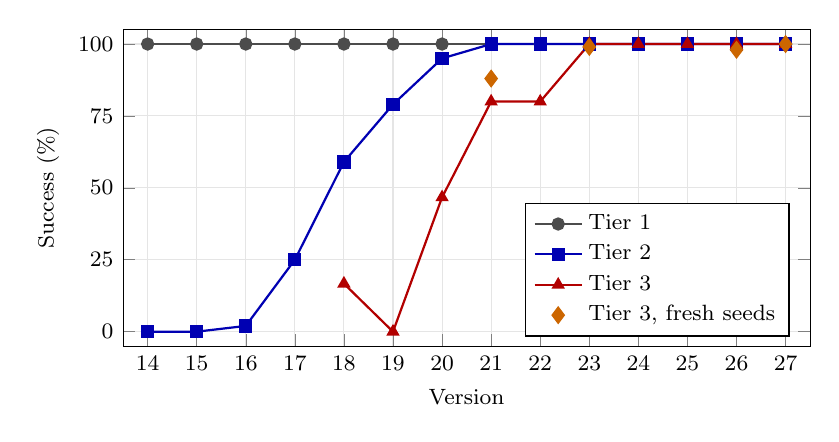
\begin{tikzpicture}
        \begin{axis}[
            width=0.85\textwidth, height=5.6cm,
            xlabel={Version}, ylabel={Success (\%)},
            xmin=13.5, xmax=27.5, ymin=-5, ymax=105,
            xtick={14,15,...,27},
            ytick={0,25,50,75,100},
            legend pos=south east, legend cell align=left,
            grid=major, grid style={black!10},
            tick label style={font=\footnotesize}, label style={font=\footnotesize}, legend style={font=\footnotesize}
        ]
            \addplot[thick, mark=*, black!70] coordinates {(14,100) (15,100) (16,100) (17,100) (18,100) (19,100) (20,100) (21,100) (22,100) (23,100) (24,100) (25,100) (26,100) (27,100)};
            \addlegendentry{Tier 1}
            \addplot[thick, mark=square*, blue!70!black] coordinates {(14,0) (15,0) (16,2) (17,25) (18,59) (19,79) (20,95) (21,100) (22,100) (23,100) (24,100) (25,100) (26,100) (27,100)};
            \addlegendentry{Tier 2}
            \addplot[thick, mark=triangle*, red!70!black] coordinates {(18,16.7) (19,0) (20,46.7) (21,80) (22,80) (23,100) (24,100) (25,100) (26,100) (27,100)};
            \addlegendentry{Tier 3}
            \addplot[only marks, mark=diamond*, mark size=3pt, orange!80!black] coordinates {(21,88) (23,99) (26,98) (27,100)};
            \addlegendentry{Tier 3, fresh seeds}
        \end{axis}
    \end{tikzpicture}
    \caption{Success on the three tiers as components were added. Version 17 ordered needs by conflicts, version 18 answered orders with the planner, version 21 introduced the effect model, and version 23 the held intention. Tier 1 stayed at 100\% throughout. Tier 3 was first run at version 18.}
    \label{fig:progress}
\end{figure}

\subsection{Commitment and information seeking carry the hardest tier}

On tier 3, the agent continued its held intention on 2,656 of 3,564 steps (75\%) and deliberated from the goal on the other 908. Every order the planner found on tiers 2 and 3 was of one kind: face the token, clearing the way to it, before changing what is carried. There were 158 such orders on tier 2, 135 on tier 3 and 592 on the fresh seeds, never the reverse, and no cycles. The surprise trigger fired 56 times on tier 3 and 183 times on the fresh seeds. In every episode its count equalled the number of the effect model's wrong predictions, consistent with every wrong prediction being noticed and leading to deliberation. The least-known-act rule chose 147 acts on tier 3 and the agent made 62 of them. By Eq.~\eqref{eq:uncertainty}, its highest scores go to boxes, whose contents the model cannot know in advance ($\eta\approx\tfrac16$), and opening them finds the keys that locked doors need.

\subsection{Deliberation stays cheap}

On tier 3, a step evaluated about 61 conditions, built 2.5 closeness fields over about 360 placements each (0.55 ms per field), and ran 1.6 order tests. A step took 11.6 ms, and the effect model's store for tier 3 held about 48,500 groups of instances. Setup, which loads random-play memory and the effect model's store and fits the moves, took 10--12.5 s per environment.

\section{Discussion}

A small set of general mechanisms solves three MiniGrid environments of increasing difficulty, ObstructedMaze-Full among them. The mechanisms are a token belief, an effect model learned from reward-free experience, backward chaining over the conditions that model exposes, commitment to the chosen chain, and acting where an outcome is least known. Several features of the results bear on how agents with world models are usually built.

First, the agent never imagines a trajectory. It imagines only the effect of one act on the tokens the act touches, and composes such effects only along a chain of conditions that leads to the goal. The work done per step is set by the number of relevant conditions, about 61 on the hardest tier, not by a horizon or a branching factor of actions. A rollout planner such as Dreamer or MuZero \cite{Hafner2025,Schrittwieser2020} imagines whole latent states and needs reward to choose among them. Here the goal is a condition in the same terms as the belief, and the effect model predicts in the encoder's latent space, as JEPA proposes \cite{LeCun2022}. But what is predicted is the abstract consequence that a plan needs (``the door becomes passable''), not the next latent state.

Second, the sample cost is small and needs no reward. The agent learned from about 3.2 million steps of uniformly random play per environment, in which a random policy happened to succeed in 0.45--5.9\% of episodes. In a published comparison on the original version of ObstructedMaze-Full, five of six reinforcement-learning methods trained with reward did not solve it, and the one that did, NovelD, reached a final test score of 0.96 \cite{Zhang2021}. Our agent's mean return on version 1 is 0.970. The comparison is not like for like. Version 1 fixes unsolvable layouts, and our agent relies on declared structure that those methods do not have: a planner, a grid-shaped belief and a goal given as a condition. What the comparison shows is that this structure turns a task that is very hard to learn from reward into one that can be solved from a few million steps of undirected experience.

Third, the agent's knowledge can be inspected. Every decision is a chain of named conditions, each backed by stored tries that can be listed. This made development a matter of tracing why a chain was chosen, not of retraining. Most components in Table~\ref{tab:versions} were found by tracing the failures of the version before.

The effect model is the part of the architecture we expect to carry over best. It follows a long tradition in which a stored instance answers a query in proportion to its similarity \cite{Medin1978,Nosofsky1986,Hintzman1986,Aha1991}. It adds three things: conditions admitted by held-out likelihood, so that irrelevant context cannot veto a memory; a network prior that takes over where experience is sparse; and results stored as relations between tokens, so that ``what was in front is now carried'' transfers to objects rarely seen. The fitted weights tell their own story. The episode's own tries override everything after a single try ($\beta\approx10^{-4}$), and the network matters only where no stored instance is near ($\alpha=0.01$). This is the division of labour that complementary learning systems predict \cite{McClelland1995,Kumaran2016}: fast, specific memory where it has evidence, slow, general structure elsewhere.

\paragraph{Limitations.} The results come with limitations that must be stated plainly.
\begin{itemize}
    \item \textbf{Perception is a lookup.} The adapter maps the simulator's cells to encoder vectors of clean renderings. The agent therefore never encodes a noisy frame while acting, segmentation into objects is given by the grid, and occlusion is computed from cell types. Several parts rely on this, for example the exact equality tests in the effect model's relations and the exact appearance identity in the episode's own tries. They would need to tolerate noise in a real image stream.
    \item \textbf{The goal and the sampling of experience use the simulator.} On tiers 2 and 3 the target object's appearance is written in from the environment. Which random-play steps were stored, and whether a stored interaction changed a token, were decided from the simulator's full state.
    \item \textbf{Many forms are declared.} These include the locus of an action as the cell ahead, a single carried slot, four outcome categories, a world that changes only by the agent's actions, the lattice sized in advance, and the settings listed in Materials and Methods.
    \item \textbf{The procedures are designed.} The search, the intention's triggers and the order of the fallbacks are designed, not learned. The three networks were trained on MiniGrid's object types.
    \item \textbf{The test seeds were not fully held out.} The test seeds were used to diagnose failures during development, and three of the fresh seeds were traced for the last two versions.
    \item \textbf{The samples are small.} Tier 3 has 30 test seeds, so differences of a few seeds there are not significant.
    \item \textbf{No reinforcement-learning baseline was run} under our protocol.
    \item \textbf{Some known failure modes remain.} The agent can plan to drop a key on the cell its route must cross; one fresh seed was won only because a held act carried it past that cell. And it can spend long stretches without a plan, as in the 1,856-step episode above.
\end{itemize}

\begin{table}[t]
    \caption{Assumptions of the agent and whether they hold beyond MiniGrid. ``Learned'' parts carry over unchanged; ``declared'' parts are environment-specific priors to be removed.}
    \centering
    \small
    \begin{tabular}{>{\raggedright\arraybackslash}p{5.2cm} >{\raggedright\arraybackslash}p{2.0cm} >{\raggedright\arraybackslash}p{5.6cm}}
        \toprule
        Assumption & Status & Beyond MiniGrid \\
        \midrule
        Moves are transformations of token positions, fitted from experience & learned & holds wherever the agent's motion is rigid in the image plane (Crafter, ARC-AGI-3); robots need 3-D transformations \\
        Effects predicted by an exemplar vote with a network prior, own tries first & learned & holds; needs tolerance to noise in place of exact equality \\
        Conditions, achievers and orders read from the effect model & learned & holds for any action with a locus \\
        Closeness by value iteration over believed placements & computed & holds on any graph of placements \\
        Patches are grid cells, one object per cell & declared & fails in Crafter's multi-tile sprites and in robotics \\
        Observation as a lookup of clean renderings & declared & fails everywhere else \\
        The locus is the cell ahead; one carried slot & declared & Crafter has an inventory of counts; ARC-AGI-3 has actions aimed at a place \\
        The world changes only by the agent's actions & declared & fails in Crafter (creatures, night) and robotics \\
        \bottomrule
    \end{tabular}
    \label{tab:portability}
\end{table}

\paragraph{Toward other environments.} Table~\ref{tab:portability} separates the parts that are general from those that are specific to MiniGrid. The goal is that a new environment should change only the adapter: frames to tokens, the list of actions and the goal. Work under way on Crafter \cite{Hafner2022} replaces the declared parts one at a time, each with a general prior:
\begin{itemize}
    \item the view's own motion is estimated from pixels with no tile, grid or agent position declared, with a likelihood tempered to count evidence per independent observation \cite{Holmes2017};
    \item objects are found as what moves together \cite{Spelke1990};
    \item objects are followed as pixel sprites \cite{Jojic2001} with earned existence and data association \cite{BarShalom1975,Musicki1994}, in the manner of object files \cite{Kahneman1992};
    \item the agent's own body is found as what its actions control.
\end{itemize}
The planner, the effect model and the intention would then run on these tokens unchanged. Whether they do, and whether conditions over learned tokens scale to Crafter's crafting chains and to the place-directed actions of ARC-AGI-3 \cite{Chollet2019}, is the test that remains.

\section*{Acknowledgments}

\subsection*{General}
During the preparation of this work, the author used Claude (Anthropic), through Claude Code, to write and run the experiment code, to keep the experiment records and to draft the manuscript. After using this tool, the author reviewed and edited the content as needed and takes full responsibility for the content of the publication.

\subsection*{Author Contributions}
A. Ricker conceived the approach, set the goals, constraints and evaluation protocol, directed and approved every experiment, and revised and approved the manuscript.

\subsection*{Funding}
% Author to complete: funding bodies and grant numbers, or the statement that the work received no specific funding.
[To be completed by the author.]

\subsection*{Competing interests}
% Author to complete.
[To be completed by the author.]

\subsection*{Data Availability}
% Author to complete: repository location and access.
The code, the per-episode results of every version and the experiment records are kept in the author's repository. [Location and access to be added by the author.]

\section*{Supplementary Materials}

No supplementary materials are submitted with this version of the manuscript.

\printbibliography

\end{document}
